\subsection{Software-Architektur}
	\subsubsection{Systemübersicht}
	Zur Übersicht über den erarbeiteten Lösungsansatz bietet sich die Darstellung durch ein Kontextdiagramm an. Darin zu erkennen sind die fünf Hauptkomponenten  DesktopViewer, CoreApp, Detector, MediaCommunication und ControllerCommunication. Weiter enthält das System mindestens drei Schnittstellen, einerseits die Bluetooth Schnittstelle zwischen Startgerät und Ballwerfer, des Weiteren muss die Kommunikation mit Kamera und Controller gewährleistet sein. Die Schnittstelle zur Kamera sollte, wenn wie geplant ein Smartphone verwendet wird, bereits durch das entsprechende Betriebssystem gegeben sein, weshalb in diesem Dokument nicht weiter auf diese Schnittstelle eingegangen wird. 
\begin{figure}[h!]
		\centering
		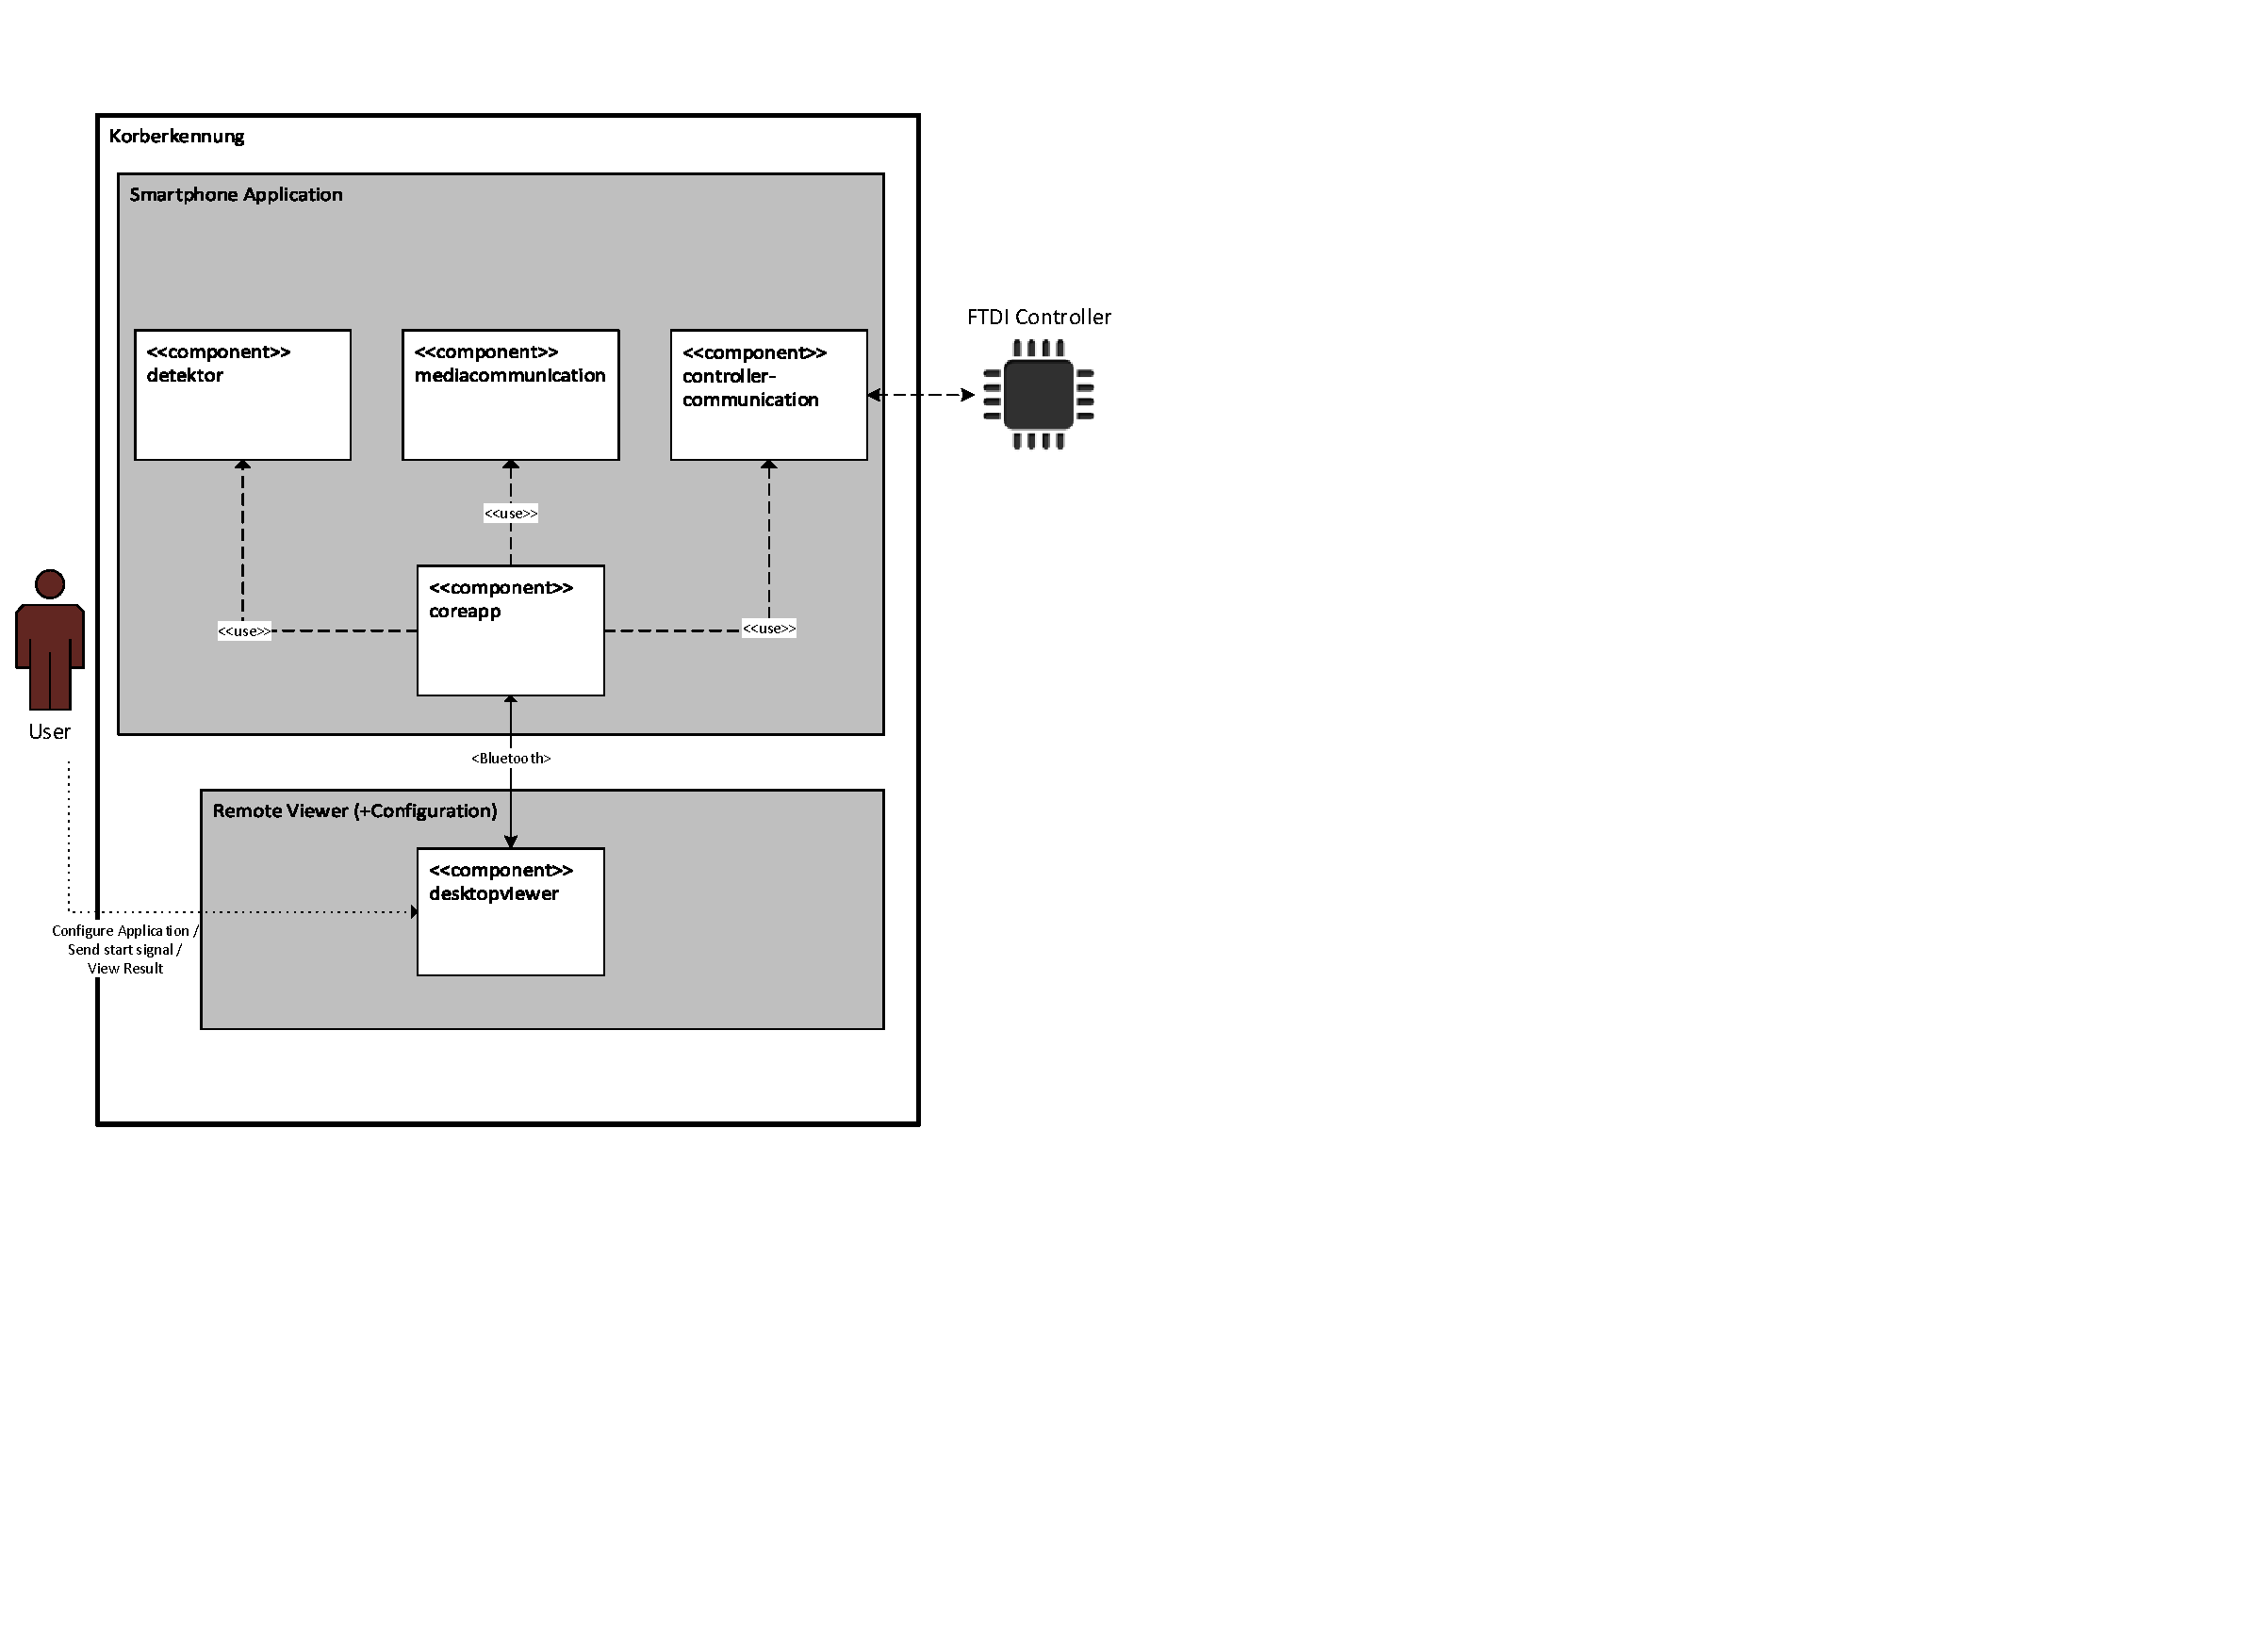
\includegraphics[width=0.9\textwidth,clip,trim= 3mm 90mm 207mm 20mm]
		{Enddokumentation/Loesungskonzept/Bilder/Kontextdiagramm_v2.pdf}
		\caption{Kontextdiagramm}		
\end{figure}
	\subsubsection{Komponenten-Spezifikation}
		\paragraph{DesktopViewer}$~~$\vspace{2mm}\\
		Über die Viewer-Komponente wird die Konfiguration der Applikation, sowie die Auslösung des Startsignals realisiert. Optional soll es zu Testzwecken möglich sein, die Resultate der Korberkennung ebenfalls über den DesktopViewer zu betrachten.
		
		\paragraph{CoreApp}$~~$\vspace{2mm}\\
		Als Kernbestandteil der Smartphone App umfasst die CoreApp-Komponente auf der einen Seite die Kommunikation mit der Viewer-Komponente, auf der anderen Seite wird hier der Ablauf der Kernfunktionen zur Objekterkennung koordiniert.		
		
		\paragraph{MediaCommunication}$~~$\vspace{2mm}\\
		In dieser Komponente ist die Kommunikation mit der Kamera des Smartphones und die Wiedergabe des Endsignals zuständig. MediaCommunication nimmt ein Foto auf und stellt dieses für die Winkelberechnung bereit, auf ein eintreffendes Endsignal wird ein Akustisches Signal ausgegeben was signalisiert das alle Bälle die Maschine verlassen haben.
		
		\paragraph{Detector}$~~$\vspace{2mm}\\
		Dem Detektor muss ein Bild übergeben werden, welches von diesem darauf ausgewertet wird. Dabei sucht der Detektor nach einem dunkeln Objekt im Bild und ist in der Lage, anhand der ermittelten Position den Winkel des Ballwerfers zum Korb bestimmen kann.
		

		\paragraph{ControllerCommunication}$~~$\vspace{2mm}\\
		Wie der Name bereits sagt wird an dieser Stelle die Kommunikation mit dem FTDI-Controller realisiert. Der vom Detektor berechnete Winkel wird hier an den FTDI-Controller übertragen. Anschliessend wartet die Komponente bis der Controller ein Endsignal zurückgibt welches das Ende des Ballwurfs signalisiert.
		
	\subsubsection{Schnittstellen-Spezifikation}
		% Übersicht Schnittstellen fehlt Schnittstellen
		\begin{figure}[h!]
			\centering
			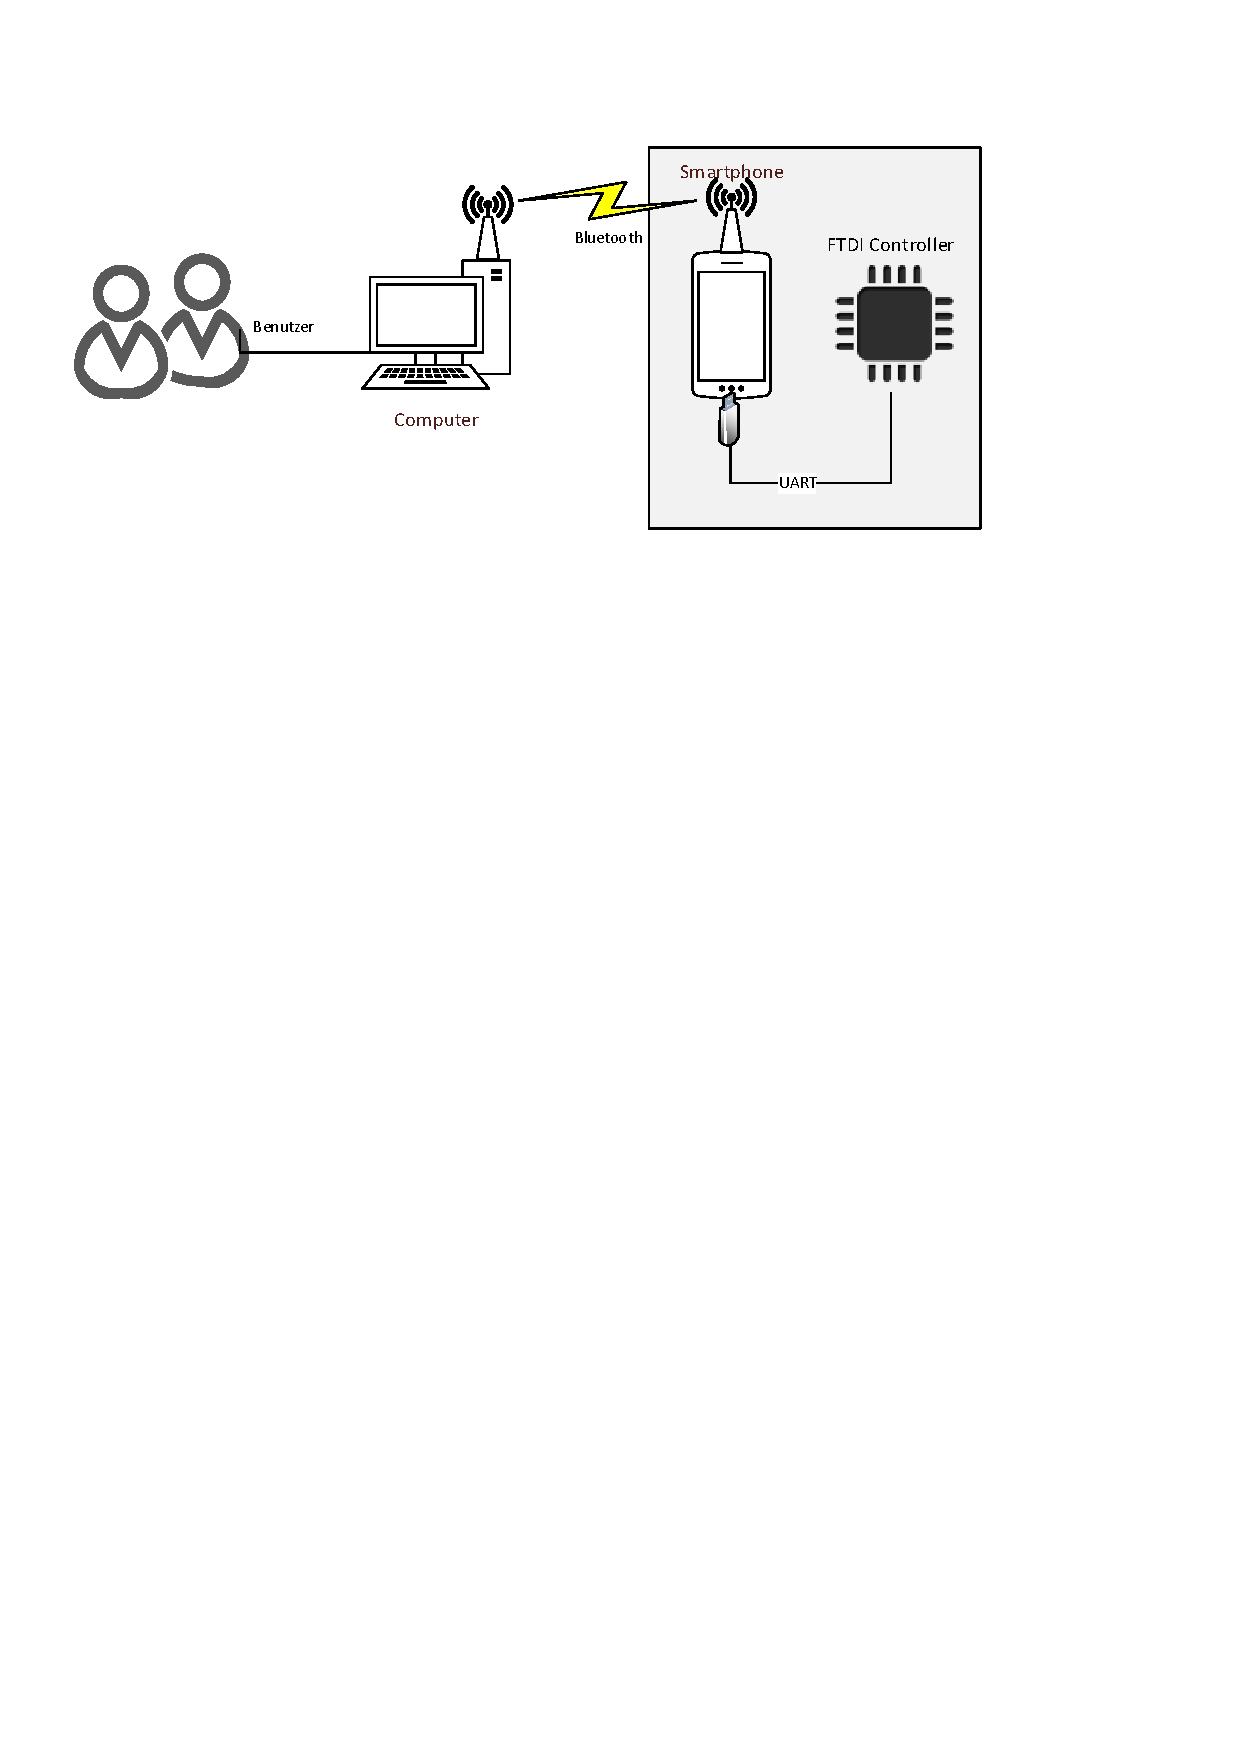
\includegraphics[width=0.9\textwidth,clip,trim= 12mm 205mm 43mm 24mm]
			{Enddokumentation/Loesungskonzept/Bilder/Schnittstellen.pdf}
			\caption{Schnittstellen}		
		\end{figure}
		Als weiteres Hauptelement des entworfenen Systems werden im nachfolgenden Abschnitt die in der Grafik erkennbaren Schnittstellen (Bluetooth und Controller) deklariert.
		\newpage
		\paragraph{Bluetooth}$~~$\vspace{2mm}\\
		Die Kommunikation vom Startgerät (Notebook) zum Smartphone (Android Device auf dem Ballwerfer) für die Übermittlung des Startsignals findet mit Bluetooth statt. Die Bluetooth-Komponente auf dem Notebook startet nach Aktivierung ein ‚inquiry‘ (Erkundigung) nach verfügbaren Bluetooth-Geräten. Anschliessend wird eine Service-Anfrage (RFCOMM, eine COM-Schnittstelle) an ein gewünschtes Bluetooth-Gerät gestartet, bei positiver Rückmeldung werden die zwei Geräte gepaart. Eine uni- oder bidirektionale Kommunikation zwischen den Geräten kann nun jederzeit aufgebaut werden. Das eigentliche Startsignal wird ein primitiver Datentyp sein.
		
		\paragraph{Controller}$~~$\vspace{2mm}\\
		Die Verbindung vom Android Smartphone zum FTDI Controller wird mit USB realisiert. 
		Das Smartphone kommuniziert über den bereitgestellten Treiber von FTDI mit dem Controller, die verwendete Schnittstelle ist UART. Die Kommunikation soll bidirektional sein, kann sowohl empfangen als auch senden. Der Vorteil einer solchen Verbindung ist, dass sie als COM-Schnittstelle angesteuert werden kann was relativ einfach zu implementieren ist. Die Verbindung ist ausfallsicher und einfach aufrechtzuerhalten.		
		
	\subsubsection{Funktionale Sicht}
	
	\begin{figure}[h!]
		\centering
		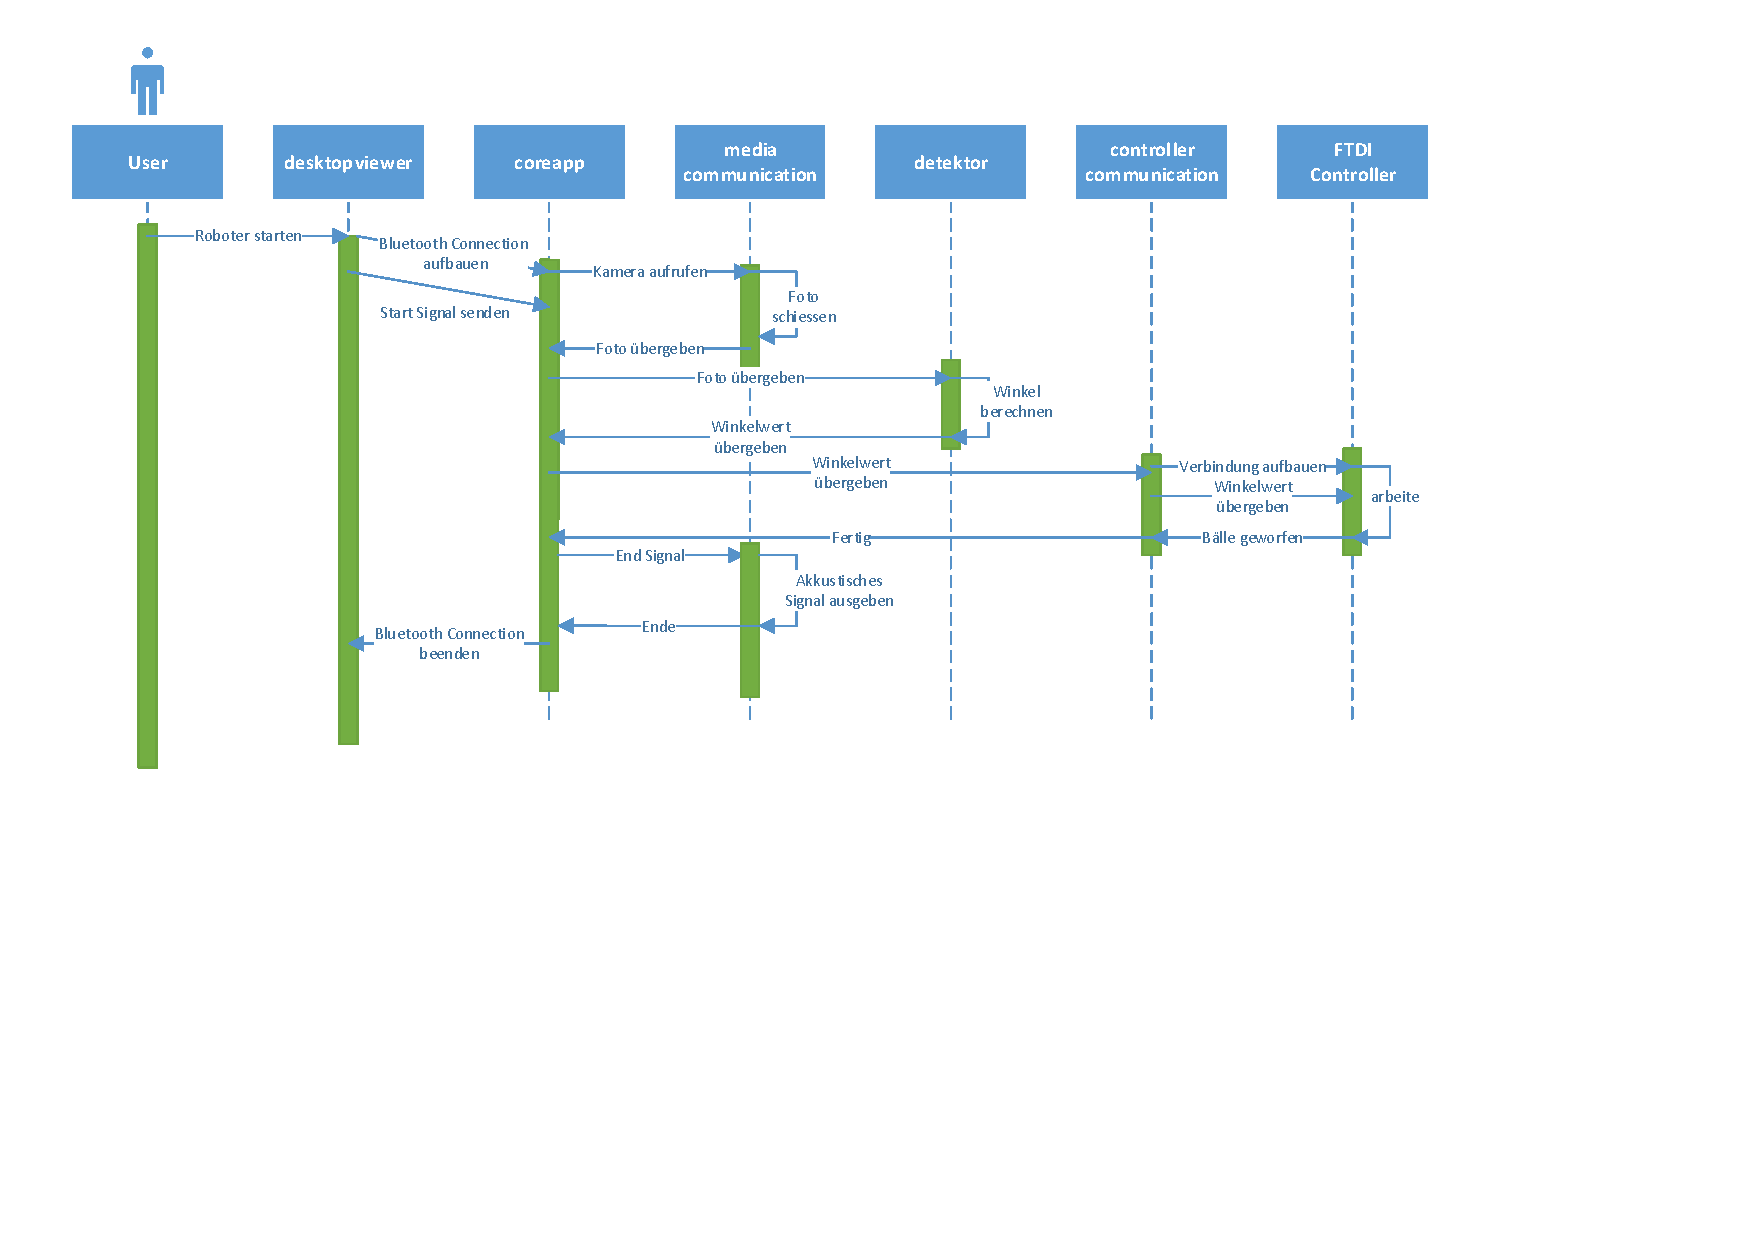
\includegraphics[width=1\textwidth,clip,trim= 11mm 88mm 55mm 8mm]
		{Enddokumentation/Loesungskonzept/Bilder/Sequenzdiagramm.pdf}
		\caption{Sequenzidagramm}		
	\end{figure}
Der Benutzer gibt den Startbefehl für den Roboter über die Komponente DesktopBiewer, die auf einem Computer(Laptop) ausgeführt wird. Der DesktopViewer baut eine Bluetooth-Verbindung mit der Komponente CoreApp auf, welche auf dem Smartphone ausgeführt wird, und sendet anschliessend das Startsignal welches durch den User ausgelöst wird. Ab diesem Zeitpunkt läuft die Applikation völlig autonom. Die CoreApp ruft als erstes die MediaCommunication Komponente auf und schiesst ein Foto. CoreApp aktiviert nun die Komponente Detector und übergibt dieser das Foto, welche daraufhin den Winkel errechnet. Der gefundene Winkel wird anschliessend an die Komponente ControllerCommunication übergeben, welche die Verbindung zum FTDI-Controller aufbaut und diesem den Winkelwert übergibt. Daraufhin wartet die Komponente bis der FTDI-Controller das Ende des Ballwurfes zurückgibt. ControllerCommunication übergibt nun an die CoreApp die Meldung, dass der Prozess beendet wurde. 
Coreapp ruft zum Schluss wiederrum die MediaCommunication Komponente auf welche das Programmende signalisiert.